\documentclass{uc3mpracticas}

\usepackage{float}

%%%%%%%%%%%%%%%%%%%%%%%%%%%%%%%%%%%%%%%%%%%%%%%%%%%%%%%%%%%%%%%%%%%%%%%%%%%%%%%%
%%%                   Plantilla Prácticas UC3M                               %%%
%%%                Universidad Carlos III de Madrid                          %%%
%%%                   Alejandro Valverde Mahou                               %%%
%%%%%%%%%%%%%%%%%%%%%%%%%%%%%%%%%%%%%%%%%%%%%%%%%%%%%%%%%%%%%%%%%%%%%%%%%%%%%%%%

%Permitir cabeceras y pie de páginas personalizados
\pagestyle{fancy}

%Declarar formato de encabezado y pie de página de las páginas del documento
\fancypagestyle{doc}{
  %Cabecera
  \headerpr[1]{Trabajo Final}{}{Aprendizaje Automático}
  %Pie de Página
  \footerpr{}{}{{\thepage} de \pageref{LastPage}}
}

%Declarar formato de encabezado y pie del título e indice
\fancypagestyle{titu}{%
  %Cabecera
  \headerpr{}{}{}
  %Pie de Página
  \footerpr{}{}{}
}


\appto\frontmatter{\pagestyle{titu}}
\appto\mainmatter{\pagestyle{doc}}


\begin{document}
  %Comienzo formato título
  \frontmatter


  %Portada 1 (Centrado todo)
  \centeredtitle{Images/SmallLogo.jpg}{Grado en Ingeniería Informática}{Curso 2019-2020}{Aprendizaje Automático}{Trabajo Final}

  \vspace{40mm}

  \authors{Alba Reinders Sánchez}{100383444}{Alejandro Valverde Mahou}{100383383}{}{}{}{}

  \newpage


  %Índice
  \tableofcontents

  \newpage

  %Comienzo formato documento general
  \mainmatter


  \section{Definición del Problema}

  El problema a resolver es la clasificación de imágenes de muestras víricas para detectar el virus \textit{SARS-CoV-2}, también conocido como \textit{COVID-19}.

  \vspace{2mm}

  Esta idea nace de una propuesta realizada para el \textit{Hackathon} de la Comunidad de Madrid '\textit{Vence al virus}', el pasado 1 y 2 de Abril. La idea es identificar los pacientes infectados a través de las muestras víricas observadas con un microoscopio TEM (\textit{Transmission Electron Microscopes}), para así conseguir una prueba rápida, efectiva y de bajo coste.

  \vspace{2mm}

  Esta prueba deberá ser capaz de reconocer si el paciente está infectado por algún virus de la familia \textit{Coronaviridae} y, dado que existen muy pocos virus de esta familia que afectan a humanos, se podría asumir con cierta probabilidad que el paciente estaría infectado con el \textit{COVID-19}.

  \vspace{3mm}

  Se ha pensado resolver este problema a través de técnicas de aprendizaje automático porque se trata de un problema de clasificación. Dado que las imágenes usadas para el entrenamiento tendrán una clase asociada, se podrán usar técnicas de \textbf{aprendizaje supervisado}. De esta forma, se reduciría el tiempo necesario para clasificar cada una de las muestras, porque eliminaría la necesidad de los especialistas de tener que revisar cada una de las muestras para comprobar si el paciente está o no infectado.

  \vspace{2mm}

  Respecto a la viabilidad de la solución propuesta, se cree que supondría una reducción de coste y tiempo respecto a los medios actuales usados para detectar este virus. Sin embargo, la obtención de las imágenes necesarias para el entrenamiento puede ser complicada, ya que el microoscopio que se requiere para obtenerlas no se encuentra en todos los laboratorios de los hospitales.

  \vspace{2mm}

  La fiabilidad que se espera obtener de esta prueba es bastante elevada puesto que se conoce que los virus de la familia \textit{Coronaviridae} poseen una característica distintiva: suelen tener forma esférica y unas púas alredor de todo su cuerpo, de forma que facilitará la diferenciación de estos virus respecto a otros.

  \vspace{3mm}

  \begin{figure}[H]
    \begin{center}
      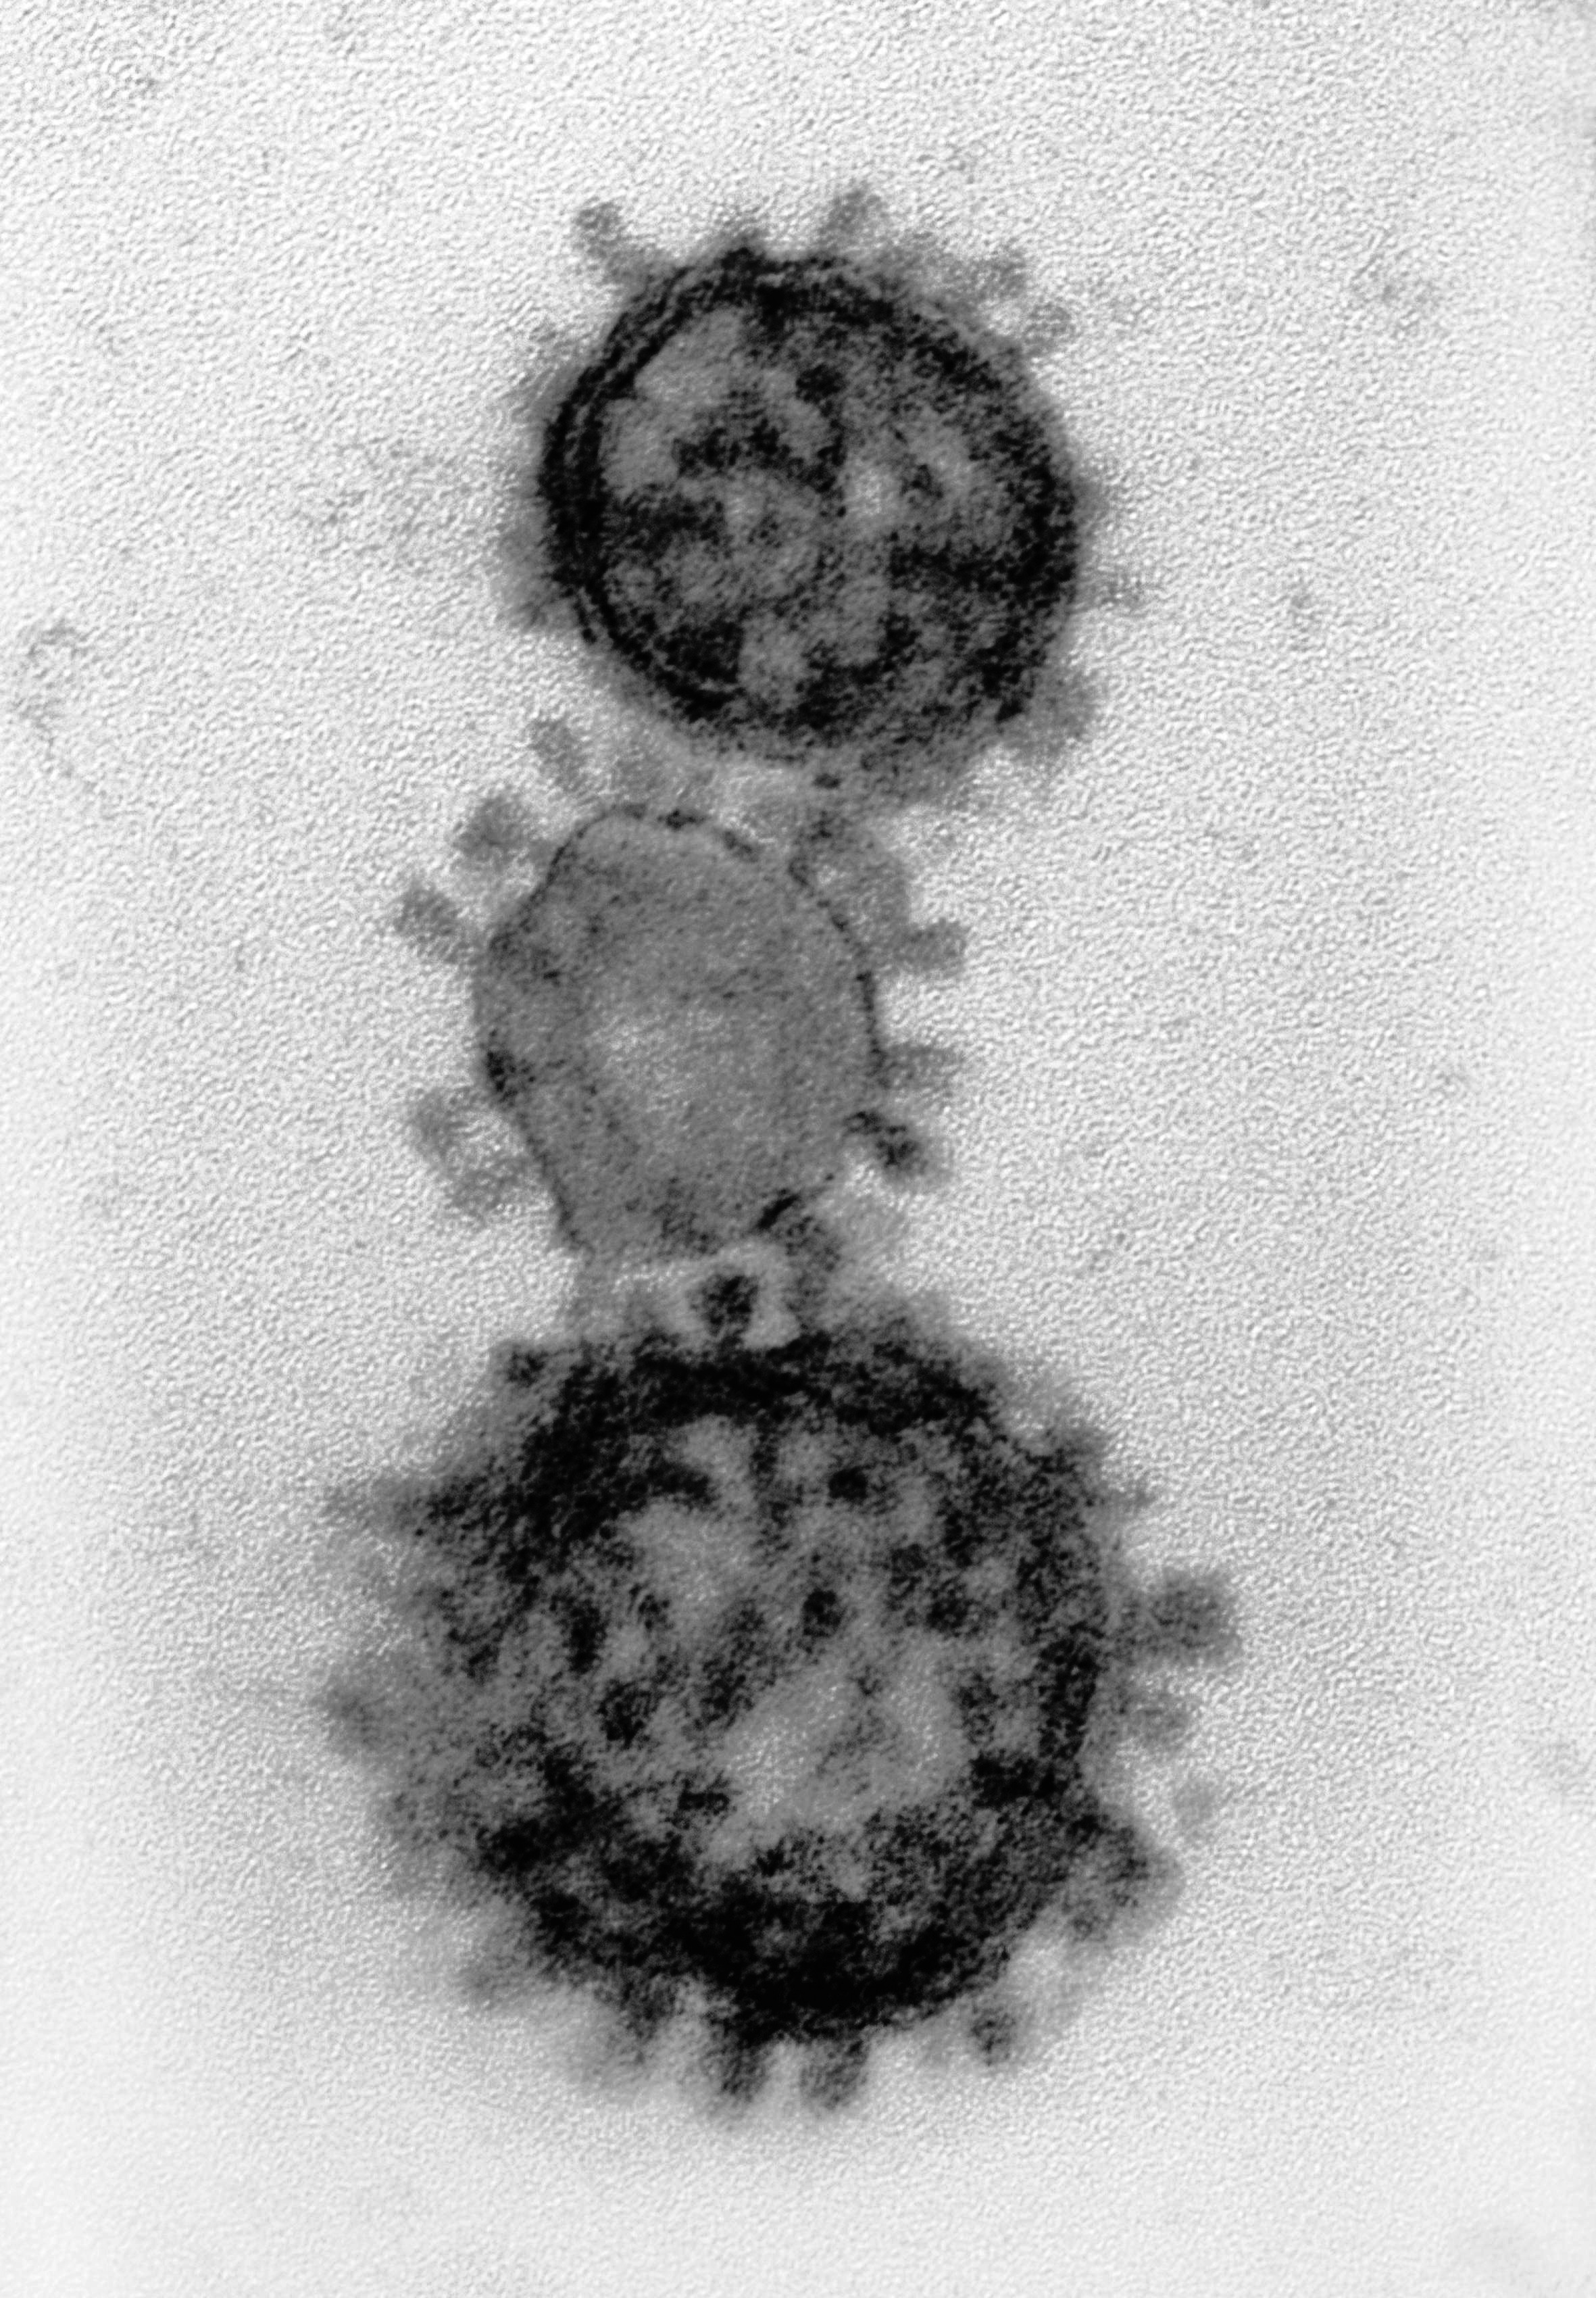
\includegraphics[angle=90,width=80mm]{Images/coronaviridae_0009.jpg}
      \caption{Muestra del virus \textit{COVID-19}}
    \end{center}
  \end{figure}

  El proceso que habría que llevar a cabo sería:

  \begin{enumerate}
    \item Recopilar un número de imágenes de muestras considerable entre las que se encuentren todo tipo de virus, entre ellos, el \textit{COVID-19}. Estas imágenes deberán estar previamente etiquetadas.
    \item Entrenar el modelo de aprendizaje automático.
    \item Evaluar el modelo generado.
    \item Utilizar este modelo para clasificar nuevas imágenes.
  \end{enumerate}

  \vspace{2mm}

  Dado que el conjunto de datos son imágenes, se va a usar una \textbf{red de neuronas} para realizar la tarea de aprendizaje automático.


% Definir el problema como una tarea de aprendizaje automático o un conjunto detareas de aprendizaje automático (en caso de que sean necesarias varias tareas)




  \section{Datos y Obtención de Datos}

  \section{Preproceso de Datos}

  \section{Modelado}

  \section{Evaluación}

  \section{Uso}








\end{document}
